\documentclass[10pt,twocolumn,letterpaper]{article}

% Page Geometry (Standard two-column dimensions: 0.75in margins, 0.25in column separation)
\usepackage[margin=0.75in,top=0.75in,bottom=1.0in,columnsep=0.25in]{geometry}

% Core Mathematical and Typography Packages
\usepackage{amsmath,amssymb,amsfonts}
\usepackage{graphicx}
\usepackage{booktabs}
\usepackage{array}
\usepackage{tabularx}
\usepackage{enumitem}
\setlist{nosep,leftmargin=1.2em}
\usepackage{url}
\usepackage{titlesec}
\usepackage{cite}
\usepackage{microtype}

\raggedbottom

% Section Heading Formatting (Standard Roman numerals, bold centered/left-aligned)
\renewcommand{\thesection}{\Roman{section}}
\renewcommand{\thesubsection}{\Alph{subsection}}
\renewcommand{\thesubsubsection}{\arabic{subsubsection}}

\titleformat{\section}{\centering\small\bfseries\scshape}{\thesection.}{0.5em}{}
\titleformat{\subsection}{\small\bfseries\itshape}{\thesubsection.}{0.5em}{}
\titleformat{\subsubsection}{\small\itshape}{\thesubsubsection)}{0.5em}{}

% Tighten spacing around section headers and equations
\titlespacing*{\section}{0pt}{9pt plus 2pt minus 2pt}{4pt plus 1pt minus 1pt}
\titlespacing*{\subsection}{0pt}{7pt plus 2pt minus 1pt}{3pt plus 1pt minus 1pt}
\titlespacing*{\subsubsection}{0pt}{5pt plus 1pt minus 1pt}{2pt plus 1pt minus 1pt}

% Title and Author Metadata
\title{\vspace{-10pt}\textbf{\LARGE Deterministic Smart Voice Keypad with Adaptive Power-Aware Preemption}\vspace{6pt}}

\author{
  \normalsize Dharmendra Yadav - 24BDS019 \qquad Suraj Ranjan Kumar - 24BDS082 \\[4pt]
  \normalsize Ravi Ranjan Bharti - 24BDS065 \qquad Rupesh Kumar - 24BDS069 \\[6pt]
  \small Department of Data Science and Artificial Intelligence
}
\date{}

\begin{document}

\maketitle

% Abstract and Index Terms Block
\begin{abstract}
\small
\textbf{\textit{Abstract}---This paper presents the end-to-end design, implementation, and empirical validation of a deterministic smart voice keypad with adaptive power-aware preemption for secure physical access control. Operating under stringent timing constraints, the architecture combines a lockless, double-buffered audio acquisition pipeline ($16$\,kHz, $16$-bit PCM) with a bounded task queue. Digital signal processing generates $40$-channel log-Mel spectrograms across $20$\,ms hops and $40$\,ms analysis windows, gated by a dynamic energy-tracking Voice Activity Detector (VAD). Keyword spotting is executed via a $28{,}693$-parameter Residual Depthwise Separable Convolutional Neural Network (Residual DS-CNN) supporting a $21$-class vocabulary ($10$ operational commands, $9$ spoken digits for PIN entry, and $2$ background classes). To ensure deadline satisfaction on edge hardware, the inference engine is subjected to systematic post-training quantization across FP32, FP16, INT16, INT8, and INT4. Symmetric per-channel INT8 quantization achieves a $4.00\times$ storage reduction ($112.08$\,KB to $28.02$\,KB), executes in $2.49$\,ms on CPU ($87.5\%$ RTOS frame margin), and maintains $93.76\%$ accuracy on $8{,}563$ held-out test samples ($99.32\%$ prediction agreement with FP32). The real-time scheduling subsystem implements and compares FIFO, Rate Monotonic (RM), and Earliest Deadline First (EDF) policies, governed by a four-state closed-loop adaptive controller that dynamically mitigates queue overloads and silence workload. The access-control subsystem enforces cryptographic PIN authentication (PBKDF2-HMAC-SHA256 with $100{,}000$ iterations), multi-tier Role-Based Access Control (RBAC), zero-latency emergency stop preemption, and immutable SQLite audit logging. The complete system is verified with $251$ automated tests and a multi-threaded WCAG-compliant web dashboard.}
\end{abstract}

\vspace{3pt}
\noindent\textbf{\textit{Index Terms}---Real-Time Systems, Keyword Spotting, Depthwise Separable CNN, Post-Training Quantization, Rate Monotonic, Earliest Deadline First, Adaptive Control, Access Control Security.}

% =========================================================================
% SECTION I: INTRODUCTION
% =========================================================================
\section{Introduction}

Voice-driven user authentication and embedded keyword spotting (KWS) have become vital components in smart building infrastructure, industrial automation, and hands-free physical security. However, conventional deep learning deployment frameworks typically prioritize unconstrained batch throughput on high-power server architectures rather than deterministic execution, bounded memory utilization, and preemption safety on edge microcontrollers.

In safety-critical access control, the software runtime must satisfy firm and hard real-time timing deadlines:
\begin{enumerate}
    \item \textbf{Audio Hop Deadline ($D_{\text{hop}} = 20$\,ms):} Audio frames arrive continuously every $20$\,ms ($50$\,Hz). Failure to process or queue an incoming block within this budget induces buffer overruns, resulting in dropped frames and acoustic phase discontinuities.
    \item \textbf{Interactive Response Deadline ($D_{\text{react}} \le 100$\,ms):} User perception and safety interlocks require sub-$100$\,ms confirmed reaction latency following the physical conclusion of a spoken access command or emergency trigger.
    \item \textbf{Zero Memory Leaks and Deterministic Execution:} Embedded edge systems lack virtual memory swap space; dynamic heap allocations inside high-priority audio ingress paths must be strictly avoided.
\end{enumerate}

To resolve these challenges, this paper presents a deterministic smart voice keypad with adaptive power-aware preemption built from fundamental mathematical principles. The core contributions of this work are:
\begin{itemize}
    \item A deterministic, lockless audio acquisition pipeline employing dual ping-pong circular buffering and bounded queue overflow management.
    \item An optimized $21$-class Residual Depthwise Separable CNN coupled with symmetric INT8 post-training quantization, cutting storage by $75\%$ while sustaining $93.76\%$ test accuracy.
    \item A formal real-time task model and schedulability analysis comparing First-In First-Out (FIFO), Rate Monotonic (RM), and Earliest Deadline First (EDF) policies.
    \item A four-state closed-loop adaptive controller that throttles redundant inferences and sheds stale workloads under transient system contention.
    \item A fail-secure smart lock finite-state machine incorporating PBKDF2-HMAC-SHA256 cryptographic hashing, multi-tier RBAC, priority emergency stop preemption, and immutable audit logging.
    \item Comprehensive empirical validation comprising $251$ passing automated regression tests, live hardware verification, and multi-profile scheduler benchmarks.
\end{itemize}

% =========================================================================
% SECTION II: SYSTEM ARCHITECTURE & AUDIO INGRESS
% =========================================================================
\section{System Architecture and Audio Ingress Pipeline}

\subsection{End-to-End Pipeline Architecture}

The system architecture follows a deterministic, unidirectional dataflow decoupled by bounded, thread-safe synchronization primitives, organized into distinct processing stages:
\begin{enumerate}
    \item \textbf{Hardware Acquisition:} Continuous physical microphone streaming into pre-allocated memory slots.
    \item \textbf{Software Ping-Pong Buffering:} Dual-buffer swapping to isolate audio interrupts from application processing.
    \item \textbf{Bounded Audio Queue:} Fixed-capacity FIFO queue enforcing explicit overflow drop policies.
    \item \textbf{DSP and Acoustic Framing:} Hann-windowed Short-Time Fourier Transform (STFT), log-Mel filterbank extraction, and dynamic Voice Activity Detection (VAD).
    \item \textbf{Real-Time Task Scheduling:} Priority-ordered task execution comparing FIFO, RM, and EDF algorithms.
    \item \textbf{Deep Learning Inference:} Quantized Residual DS-CNN forward pass and softmax confidence smoothing.
    \item \textbf{Command State Machine:} Multi-stage confirmation gating with candidate thresholding, margin checking, and cooldown suppression.
    \item \textbf{Access Security and Lock Control:} Cryptographic PIN matching, RBAC enforcement, lockout management, and emergency preemption.
    \item \textbf{Telemetry and Web Dashboard:} Asynchronous audit persistence and live HTTP telemetry streaming.
\end{enumerate}

\subsection{Audio Acquisition Parameters}

The physical audio ingress subsystem interfaces with the host audio abstraction layer (PortAudio), capturing single-channel audio at $16{,}000$\,samples per second with $16$-bit signed integer resolution (PCM16):
\begin{equation}
    f_s = 16{,}000\,\text{Hz}, \quad T_s = \frac{1}{f_s} = 62.5\,\mu\text{s}.
\end{equation}
Audio frames are partitioned into two fundamental timing intervals:
\begin{itemize}
    \item \textbf{Hop Size ($H$):} $320$\,samples ($20.0$\,ms), establishing the periodic execution cadence ($f_{\text{hop}} = 50$\,Hz).
    \item \textbf{Window Size ($W$):} $640$\,samples ($40.0$\,ms), spanning two consecutive hops to yield a $50\%$ overlap for spectral leakage suppression.
\end{itemize}

\subsection{Ping-Pong Double Buffering Mechanism}

To prevent race conditions between the audio hardware callback and consumer processing threads, a software ping-pong double buffer is deployed. Let $B_0$ and $B_1$ represent two pre-allocated NumPy arrays of size $H = 320$. While the audio acquisition callback writes into active buffer $B_k$, the consumer thread extracts data from inactive buffer $B_{1-k}$. Upon completion of exactly $H$ samples, an atomic buffer switch occurs:
\begin{equation}
    k \leftarrow (k \oplus 1), \quad \tau_{\text{switch}} = t_{\text{now}}.
\end{equation}
This handoff executes in $\mathcal{O}(1)$ time without holding heap allocation locks or blocking the audio stream.

\subsection{Bounded Queue and Overrun Protection}

Extracted hops are pushed into a bounded audio queue with fixed capacity $Q_{\text{cap}} = 100$\,blocks ($2.0$\,s total audio capacity). Under transient operating system load spikes where the queue reaches capacity ($Q_{\text{occ}} = Q_{\text{cap}}$), the queue executes an explicit \textit{Drop-Oldest Non-Blocking Policy}:
\begin{equation}
    b_{\text{dropped}} \leftarrow Q.\text{pop\_front}(), \quad Q.\text{push\_back}(b_{\text{new}}).
\end{equation}
This policy ensures that the freshest acoustic frame is always retained for processing, avoiding latency accumulation (bufferbloat) and guaranteeing that voice commands are evaluated with minimum delay.

% =========================================================================
% SECTION III: ACOUSTIC DSP & ADAPTIVE VAD
% =========================================================================
\section{Acoustic DSP and Adaptive Voice Activity Detection}

\subsection{Windowing and Power Spectral Density}

Each analysis window of $N = 640$\,samples is tapered using a discrete periodic Hann window function $w[n]$ to minimize spectral sidelobes:
\begin{equation}
    w[n] = 0.5 - 0.5 \cos\left(\frac{2\pi n}{N}\right), \quad 0 \le n < N.
\end{equation}
The windowed discrete signal $x_w[n] = x[n] \cdot w[n]$ is transformed into the frequency domain via a $512$-point Fast Fourier Transform (FFT) with zero-padding to $N_{\text{fft}} = 1024$:
\begin{equation}
    X[k] = \sum_{n=0}^{N_{\text{fft}}-1} \tilde{x}_w[n] e^{-j \frac{2\pi}{N_{\text{fft}}} kn}, \quad 0 \le k \le \frac{N_{\text{fft}}}{2}.
\end{equation}
The single-sided power spectral density $P[k]$ is computed as:
\begin{equation}
    P[k] = \frac{1}{N_{\text{fft}}} |X[k]|^2.
\end{equation}

\subsection{Log-Mel Filterbank Energy Extraction}

Human auditory perception adheres to a non-linear logarithmic pitch scale. Frequencies are mapped to the Mel scale via:
\begin{equation}
    m = 2595 \log_{10}\left(1 + \frac{f}{700}\right).
\end{equation}
A triangular filterbank comprising $M = 40$ overlapping bandpass filters $H_m[k]$ spanning $f_{\text{low}} = 20$\,Hz to $f_{\text{high}} = 4{,}000$\,Hz is applied to the power spectrum:
\begin{equation}
    E[m] = \sum_{k} P[k] \cdot H_m[k], \quad 1 \le m \le 40.
\end{equation}
To match human dynamic range perception, log-Mel energies are calculated:
\begin{equation}
    S[m] = \ln(E[m] + \epsilon), \quad \epsilon = 10^{-6}.
\end{equation}
A rolling circular context window collects $T = 49$ consecutive hops ($980$\,ms context), producing a feature tensor $\mathbf{X}$ (1 input channel, 49 time frames, 40 Mel bins):
\begin{equation}
    \mathbf{X} \in \mathbb{R}^{1 \times 49 \times 40}.
\end{equation}

% Figure 1: DSP Feature Extraction Plot (Spans Both Columns)
\begin{figure*}[t]
    \centering
    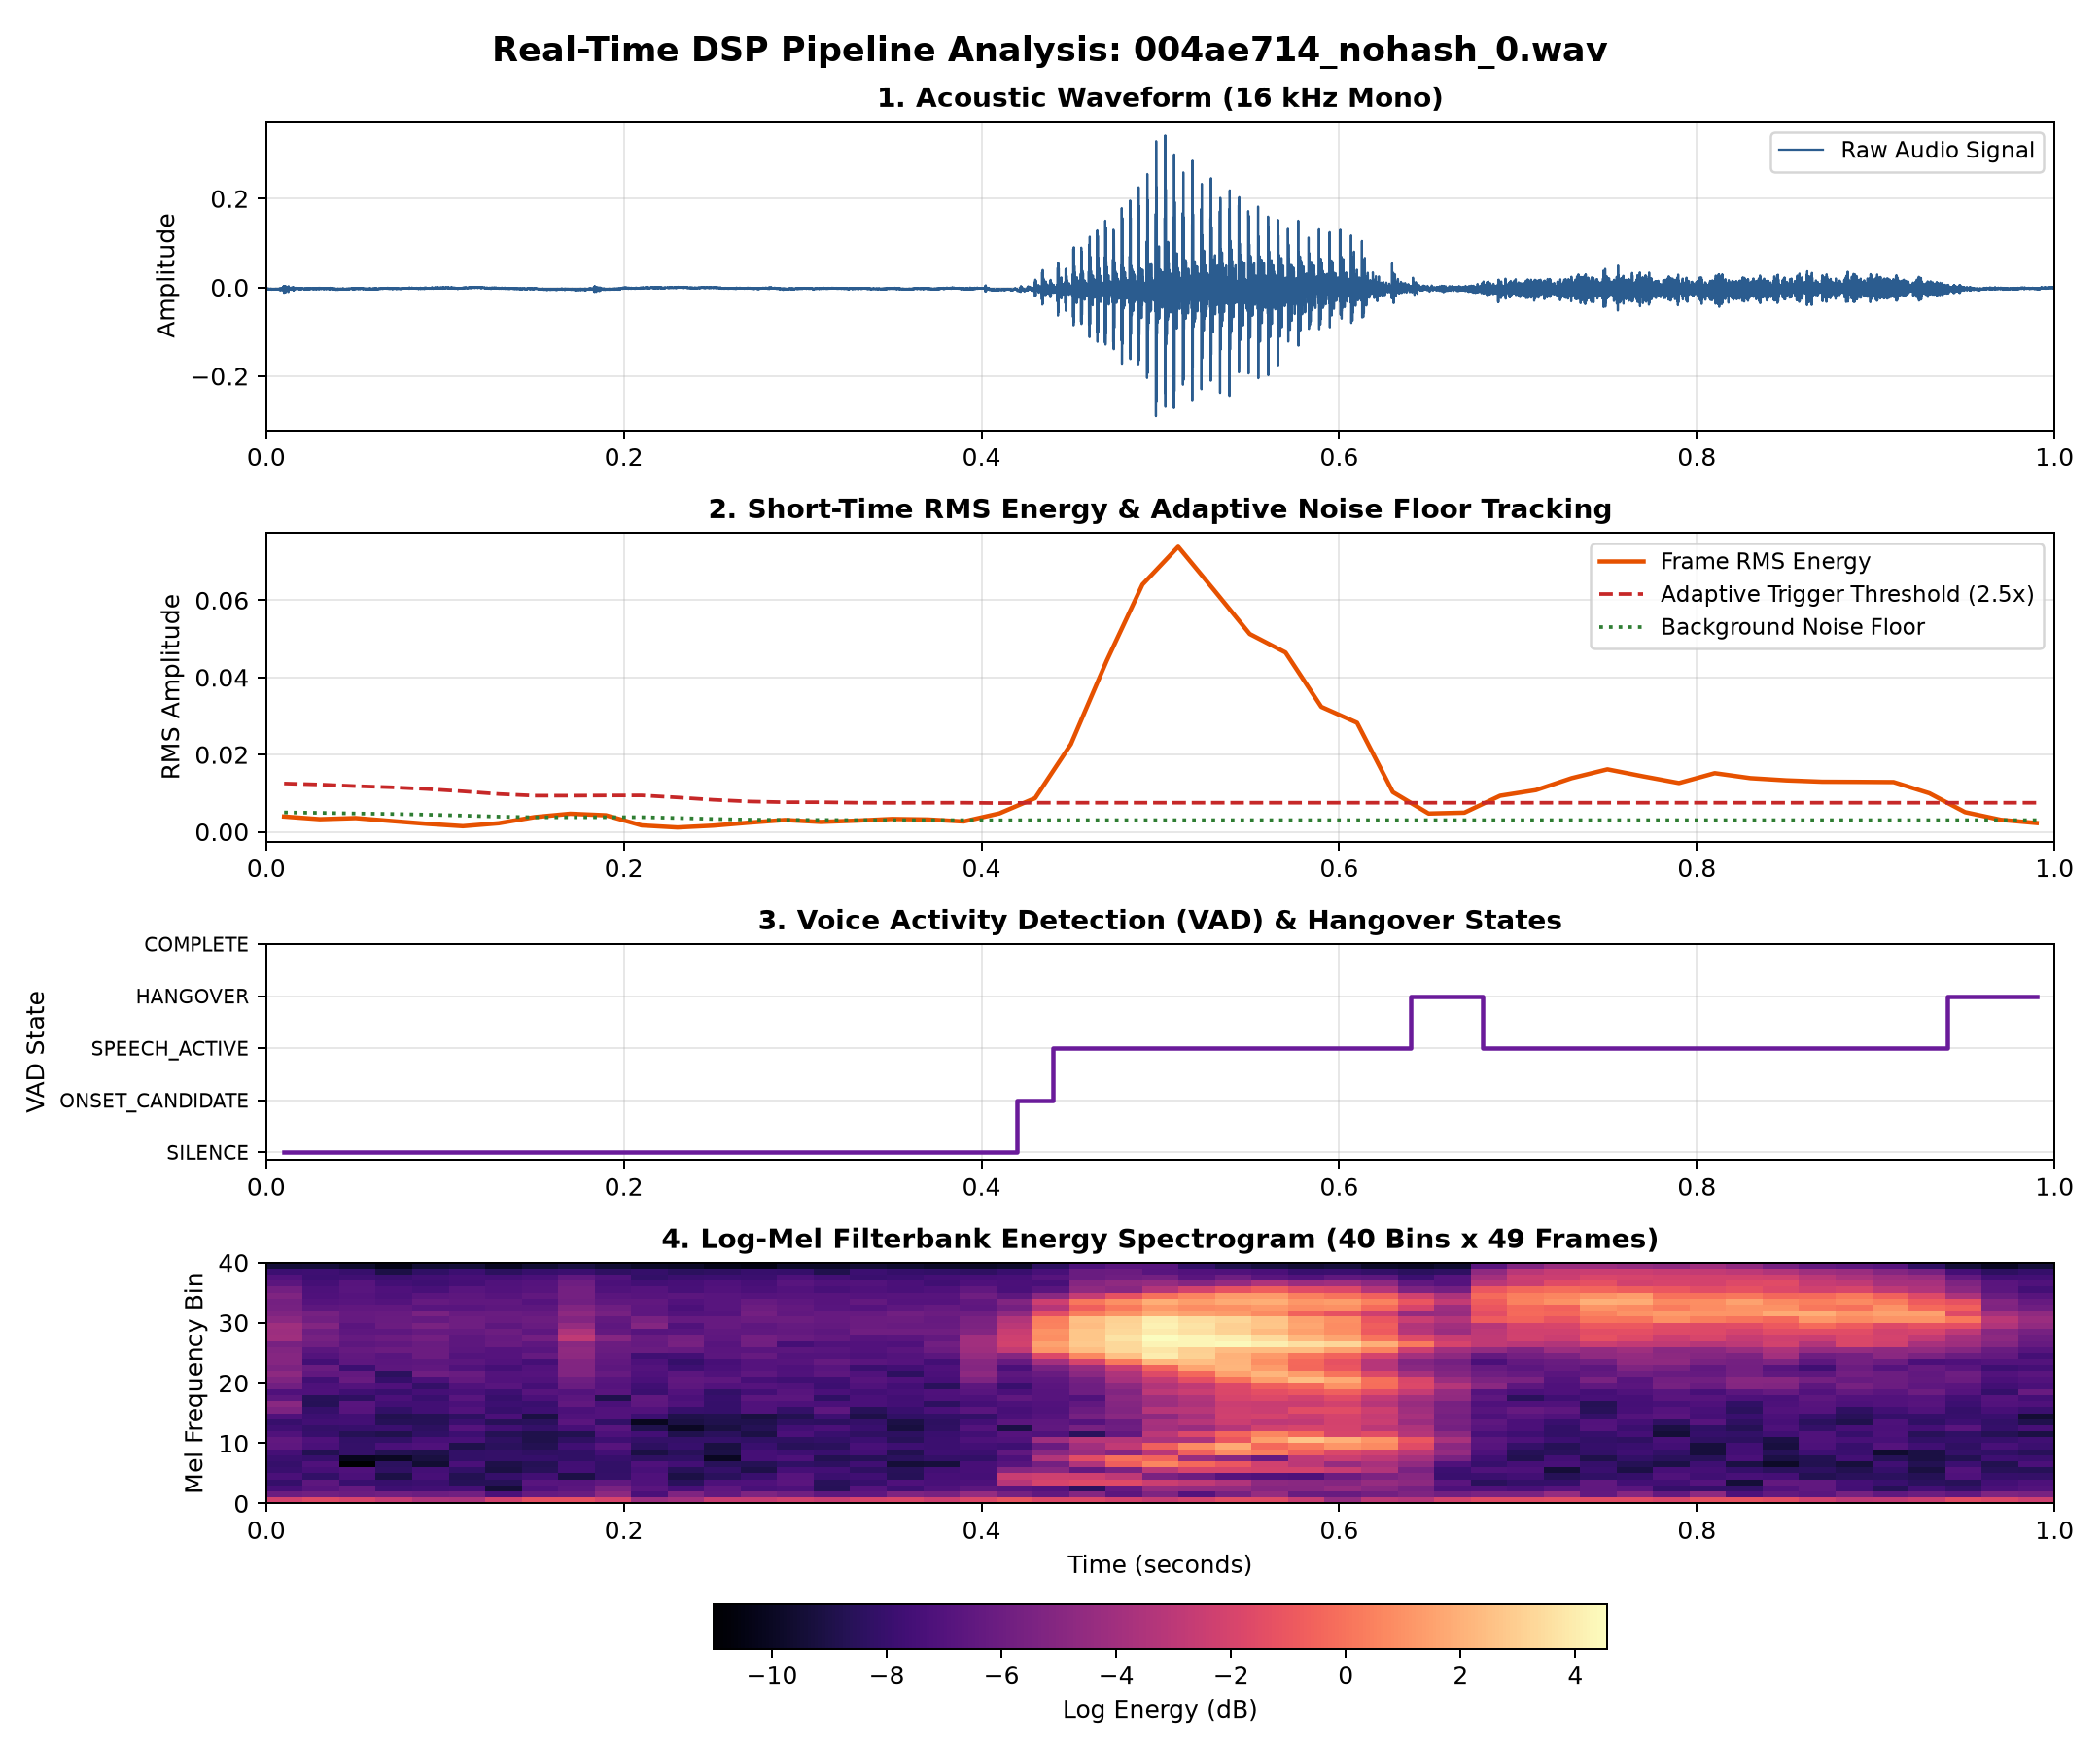
\includegraphics[width=0.96\textwidth]{figures/dsp_visualization.png}
    \caption{Acoustic digital signal processing pipeline: (a) Input raw PCM16 audio waveform, (b) 512-point STFT spectrogram, (c) 40-channel log-Mel filterbank feature representations across 49 temporal hops, and (d) Energy tracking with dual-threshold Voice Activity Detection.}
    \label{fig:dsp_pipeline}
\end{figure*}

\subsection{Dynamic Noise Floor and Dual-Threshold VAD}

To prevent executing unnecessary neural network inference during ambient room silence, an energy-based Voice Activity Detector computes the short-term Root Mean Square (RMS) energy:
\begin{equation}
    \text{RMS} = \sqrt{\frac{1}{W} \sum_{n=0}^{W-1} x^2[n]}.
\end{equation}
The background noise floor $\sigma_{\text{noise}}$ dynamically adapts during quiet periods using an asymmetric exponential moving average:
\begin{equation}
    \sigma_{\text{noise}}^{(t)} = \alpha \sigma_{\text{noise}}^{(t-1)} + (1 - \alpha) \text{RMS},
\end{equation}
where $\alpha = 0.98$ for rising noise (slow upward adaptation) and $\alpha = 0.90$ for falling noise (rapid quiet tracking).

State transitions follow a dual-threshold hysteresis rule:
\begin{equation}
    S_{\text{VAD}} = 
    \begin{cases}
        \text{SPEECH}, & \text{RMS} \ge 3.5\,\sigma_{\text{noise}}, \\
        \text{SILENCE}, & \text{RMS} < 1.8\,\sigma_{\text{noise}} \text{ for } 300\,\text{ms}, \\
        \text{HOLD}, & \text{otherwise}.
    \end{cases}
\end{equation}
A $200$\,ms circular pre-roll buffer ($3{,}200$\,samples) continuously stores preceding audio, ensuring that initial plosive consonants (e.g., /t/ in ``two'', /f/ in ``four'') are fully captured upon speech onset.

% =========================================================================
% SECTION IV: RESIDUAL DS-CNN & QUANTIZATION
% =========================================================================
\section{Edge Neural Keyword Spotting and INT8 Quantization}

\subsection{Residual Depthwise Separable CNN Formulation}

Standard 2D convolutions jointly filter spatial coordinates and cross-channel correlations, requiring high parameter counts and computational operations. A depthwise separable convolution factorizes this operation into:
\begin{enumerate}
    \item \textbf{Depthwise 2D Convolution:} Applies a single spatial/frequency filter per input channel without cross-channel mixing.
    \item \textbf{Pointwise $1 \times 1$ Convolution:} Computes linear combinations across all depthwise channels.
\end{enumerate}

For an input feature map $\mathbf{F} \in \mathbb{R}^{D_F \times D_F \times M}$ and output channels $N$, using kernel size $D_K \times D_K$, the computational cost comparison is:
\begin{align}
    C_{\text{std}} &= D_K^2 \cdot M \cdot N \cdot D_F^2, \\
    C_{\text{DS}} &= D_K^2 \cdot M \cdot D_F^2 + M \cdot N \cdot D_F^2.
\end{align}
The theoretical reduction factor in arithmetic complexity is:
\begin{equation}
    \frac{C_{\text{DS}}}{C_{\text{std}}} = \frac{1}{N} + \frac{1}{D_K^2} \approx \frac{1}{64} + \frac{1}{9} \approx 0.126,
\end{equation}
achieving an $87.4\%$ reduction in computational overhead.

To prevent vanishing gradients, identity residual skip connections are added across all depthwise blocks:
\begin{equation}
    \mathbf{y} = \mathbf{x} + \mathcal{F}(\mathbf{x}, \{W_i\}),
\end{equation}
where $\mathcal{F}$ represents Depthwise Conv, BatchNorm, ReLU, Pointwise Conv, BatchNorm, and Dropout ($p = 0.10$). The structural breakdown is detailed in Table~\ref{tab:model_architecture}.

\begin{table}[htbp]
\centering
\footnotesize
\setlength{\tabcolsep}{3pt}
\caption{Detailed Structural Breakdown of Residual DS-CNN}
\label{tab:model_architecture}
\begin{tabularx}{\columnwidth}{lXr}
\toprule
\textbf{Layer / Block} & \textbf{Output Shape} & \textbf{Params} \\
\midrule
Input Spectrogram & $(1, 49, 40)$ & 0 \\
Initial Conv2D ($10 \times 4, s=2$) & $(64, 25, 20)$ & $2{,}688$ \\
DS-Block 1 (Res, $3 \times 3$) & $(64, 25, 20)$ & $4{,}928$ \\
DS-Block 2 (Res, $3 \times 3$) & $(64, 25, 20)$ & $4{,}928$ \\
DS-Block 3 (Res, $3 \times 3$) & $(64, 25, 20)$ & $4{,}928$ \\
DS-Block 4 (Res, $3 \times 3$) & $(64, 25, 20)$ & $4{,}928$ \\
DS-Block 5 (Res, $3 \times 3$) & $(64, 25, 20)$ & $4{,}928$ \\
Adaptive AvgPool ($1 \times 1$) & $(64, 1, 1)$ & 0 \\
Classifier Linear ($64 \rightarrow 21$) & $(21)$ & $1{,}365$ \\
\midrule
\textbf{Total Parameters} & \textbf{28,693 Trainable} & \textbf{112.1\,KB} \\
\bottomrule
\end{tabularx}
\end{table}

\subsection{21-Class Target Vocabulary}

The deployed classifier operates on $C = 21$ discrete speech categories:
\begin{itemize}
    \item \textbf{10 Operational Commands:} \texttt{yes}, \texttt{no}, \texttt{up}, \texttt{down}, \texttt{left}, \texttt{right}, \texttt{on}, \texttt{off}, \texttt{stop}, \texttt{go}.
    \item \textbf{9 Spoken PIN Digits:} \texttt{one}, \texttt{two}, \texttt{three}, \texttt{four}, \texttt{five}, \texttt{six}, \texttt{seven}, \texttt{eight}, \texttt{nine} (the digit \texttt{zero} is omitted to prevent acoustic confusion with the letter `o' and \texttt{no}).
    \item \textbf{2 Background Classes:} \texttt{\_silence\_} (ambient acoustic noise) and \texttt{\_unknown\_} (out-of-vocabulary words).
\end{itemize}

\subsection{Post-Training Quantization Formulation}

To deploy onto memory-constrained microcontrollers, the model weights $W$ undergo uniform symmetric per-channel affine quantization. For bitwidth $b \in \{32, 16, 8, 4\}$, the integer range is:
\begin{equation}
    q_{\min} = -2^{b-1}, \quad q_{\max} = 2^{b-1} - 1.
\end{equation}
The per-channel scaling factor $\Delta_c$ is determined by the absolute peak tensor weight across output channel $c$:
\begin{equation}
    \Delta_c = \frac{\max_j |W_{c,j}|}{q_{\max}}.
\end{equation}
Quantized weights $W_{q,c}$ and their reconstructed floating-point representations $\hat{W}_c$ are computed as:
\begin{align}
    W_{q,c} &= \text{clamp}\left(\text{round}\left(\frac{W_c}{\Delta_c}\right), q_{\min}, q_{\max}\right), \\
    \hat{W}_c &= W_{q,c} \cdot \Delta_c.
\end{align}

% Table 2: Master Quantization Benchmark (Spans Both Columns)
\begin{table*}[t]
\centering
\small
\caption{Master Quantization Benchmark Across 8,563 Held-Out Speech Test Samples}
\label{tab:quantization_benchmark}
\begin{tabular}{lccccc}
\toprule
\textbf{Metric} & \textbf{FP32} & \textbf{FP16} & \textbf{INT16} & \textbf{INT8 (Selected)} & \textbf{INT4} \\
\midrule
Numerical Precision & 32-bit Float & 16-bit Float & 16-bit Int & \textbf{8-bit Int} & 4-bit Int \\
Weight Storage Size (KB) & $112.08$ & $56.04$ & $56.04$ & \textbf{28.02} & $14.01$ \\
Compression Ratio & $1.00\times$ & $2.00\times$ & $2.00\times$ & $\mathbf{4.00\times}$ & $8.00\times$ \\
Peak RAM Footprint (KB) & $362.08$ & $181.04$ & $306.04$ & \textbf{278.02} & $264.01$ \\
\midrule
\textbf{Test Accuracy (8,563 Samples)} & \textbf{94.01\%} & \textbf{94.01\%} & \textbf{94.01\%} & \textbf{93.76\%} & $82.96\%$ \\
Accuracy Delta vs. FP32 Baseline & $\pm 0.00\%$ & $\pm 0.00\%$ & $\pm 0.00\%$ & $\mathbf{-0.25\%}$ & $-11.05\%$ \\
Prediction Agreement with FP32 & $100.00\%$ & $99.98\%$ & $100.00\%$ & \textbf{99.32\%} & $85.08\%$ \\
Logit Cosine Similarity & $1.000000$ & $0.999998$ & $1.000000$ & \textbf{0.999589} & $0.797008$ \\
Signal-to-Quantization-Noise Ratio (SQNR) & $121.20$\,dB & $53.94$\,dB & $77.40$\,dB & \textbf{28.23\,dB} & $1.19$\,dB \\
\midrule
Mean CPU Latency & $2.70$\,ms & $41.70$\,ms & $2.85$\,ms & \textbf{2.49\,ms} & $2.58$\,ms \\
Median (P50) Latency & $2.56$\,ms & $41.42$\,ms & $2.71$\,ms & \textbf{2.38\,ms} & $2.44$\,ms \\
95th Percentile (P95) Latency & $3.99$\,ms & $47.99$\,ms & $4.26$\,ms & \textbf{3.46\,ms} & $3.66$\,ms \\
Throughput (Inferences / Second) & $370.7$ & $24.0$ & $351.5$ & \textbf{401.0} & $388.2$ \\
\midrule
\textbf{RTOS 20\,ms Frame Deadline Margin} & $\mathbf{+86.5\%}$ & \textbf{VIOLATED} & $\mathbf{+85.8\%}$ & $\mathbf{+87.5\%}$ & $+87.1\%$ \\
\bottomrule
\end{tabular}
\end{table*}

\subsection{Quantization Benchmark Results}

Table~\ref{tab:quantization_benchmark} summarizes the empirical quantization benchmark across all $8{,}563$ official test samples:
\begin{itemize}
    \item \textbf{INT8 Optimality:} INT8 reduces weight storage by $75\%$ ($28.02$\,KB) with a negligible accuracy drop of $0.25\%$ ($93.76\%$), while achieving $99.32\%$ classification agreement with unquantized FP32 and an SQNR of $28.23$\,dB. Mean latency drops to $2.49$\,ms on CPU due to reduced cache thrashing, yielding an $87.5\%$ safety margin below the $20$\,ms frame budget.
    \item \textbf{Hardware Breakdown of FP16 on x86:} While FP16 reduces storage, latency surges to $41.70$\,ms ($15\times$ slowdown) due to lack of native AVX-512 FP16 arithmetic units on standard consumer CPUs, violating the real-time frame deadline by $108\%$.
    \item \textbf{Failure of Naive INT4:} INT4 exhibits a severe accuracy drop to $82.96\%$ ($-11.05\%$) and an unusable $1.19$\,dB SQNR. Small $3 \times 3$ depthwise filters contain only $9$ parameters per channel; partitioning them into $16$ discrete bins severely impairs frequency discrimination.
\end{itemize}

Figure~\ref{fig:confusion_matrix} displays the normalized 21-class confusion matrix for the INT8 model, demonstrating high diagonal concentration across commands and digits.

\begin{figure}[t]
    \centering
    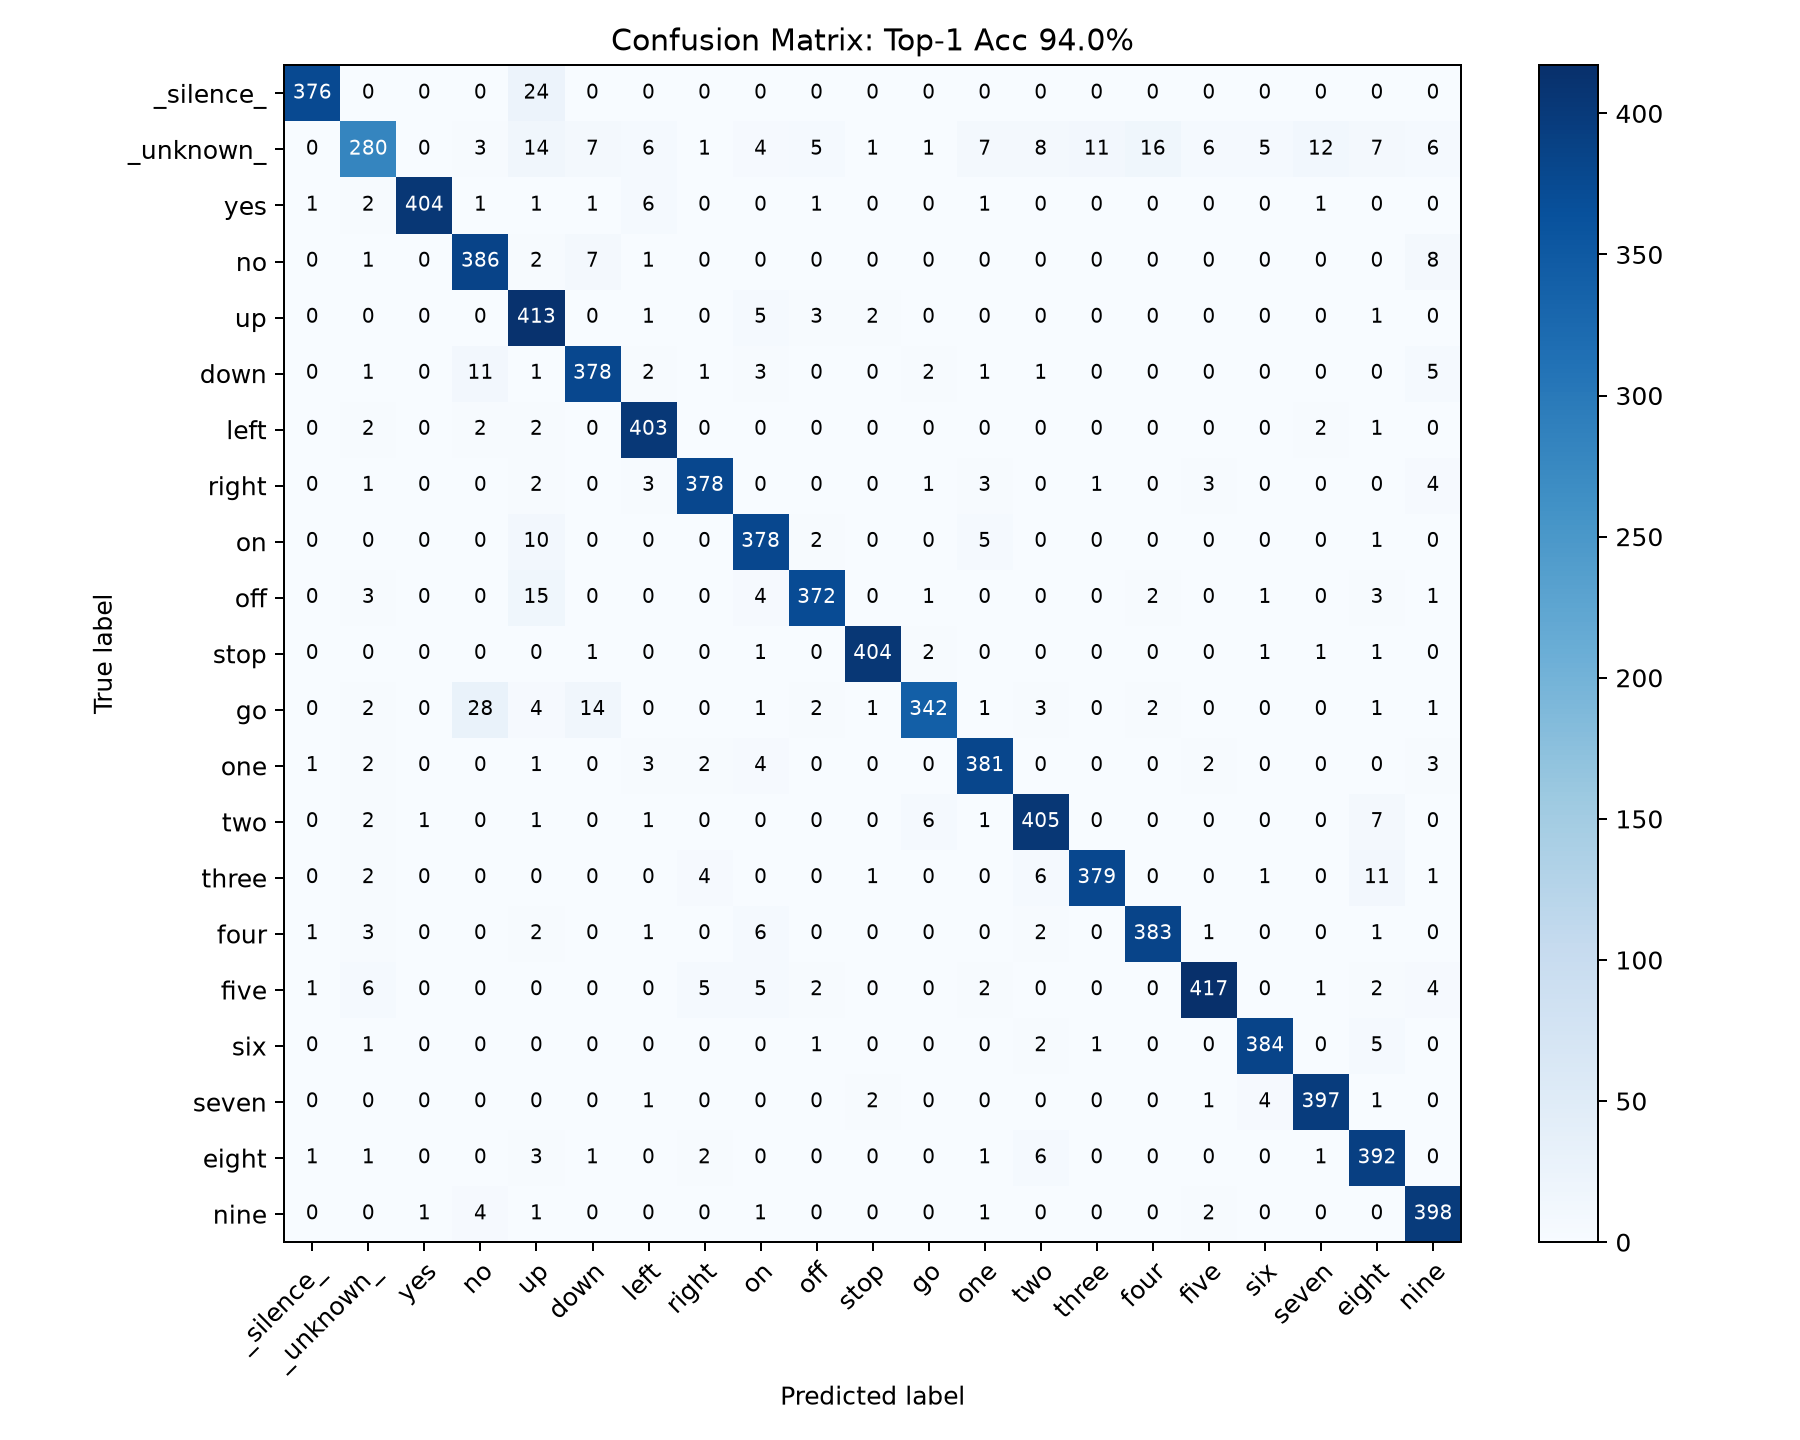
\includegraphics[width=0.92\columnwidth]{figures/confusion_matrix.png}
    \caption{Normalized confusion matrix of the 21-class quantized INT8 Residual DS-CNN evaluated on 8,563 held-out test audio samples.}
    \label{fig:confusion_matrix}
\end{figure}

% =========================================================================
% SECTION V: REAL-TIME SCHEDULING ANALYSIS
% =========================================================================
\section{Real-Time Task Scheduling Analysis}

\subsection{Formal Real-Time Task Model}

The system defines a periodic and sporadic real-time task set $\mathcal{T} = \{\tau_{\text{audio}}, \tau_{\text{dsp}}, \tau_{\text{infer}}, \tau_{\text{ctrl}}\}$. Each task $\tau_i$ is formally characterized by the 3-tuple:
\begin{equation}
    \tau_i = (C_i, T_i, D_i),
\end{equation}
where $C_i$ denotes worst-case execution time (WCET), $T_i$ is the invocation period, and $D_i$ is the relative deadline:
\begin{itemize}
    \item $\tau_{\text{audio}}$ (Ingress \& Buffering): $C_1 = 0.2$\,ms, $T_1 = 20$\,ms, $D_1 = 20$\,ms.
    \item $\tau_{\text{dsp}}$ (STFT \& Log-Mel): $C_2 = 0.6$\,ms, $T_2 = 20$\,ms, $D_2 = 20$\,ms.
    \item $\tau_{\text{infer}}$ (INT8 DS-CNN): $C_3 = 2.5$\,ms, $T_3 = 20$\,ms, $D_3 = 20$\,ms.
    \item $\tau_{\text{ctrl}}$ (FSM \& Smart Lock): $C_4 = 0.1$\,ms, $T_4 = 20$\,ms, $D_4 = 20$\,ms.
\end{itemize}

The cumulative CPU utilization factor $U$ is:
\begin{equation}
    U = \sum_{i=1}^{4} \frac{C_i}{T_i} = \frac{0.2}{20} + \frac{0.6}{20} + \frac{2.5}{20} + \frac{0.1}{20} = \frac{3.4}{20} = 0.170.
\end{equation}
The baseline utilization of $17.0\%$ provides substantial headroom for background telemetry and operating system scheduling jitter.

\subsection{Schedulability Analysis: RM vs. EDF}

Two priority-based real-time scheduling algorithms are analyzed:
\begin{enumerate}
    \item \textbf{Rate Monotonic (RM):} Static priority assignment inversely proportional to task period ($T_i$). For identical periods ($T_i = 20$\,ms), priority is assigned statically: $\tau_{\text{audio}} > \tau_{\text{dsp}} > \tau_{\text{infer}} > \tau_{\text{ctrl}}$. By the Liu and Layland utilization bound theorem:
    \begin{equation}
        U \le n(2^{1/n} - 1) = 4(2^{1/4} - 1) \approx 0.756.
    \end{equation}
    Because $U = 0.170 \le 0.756$, the task set is provably schedulable under Rate Monotonic scheduling.
    \item \textbf{Earliest Deadline First (EDF):} Dynamic priority assignment where the active job with the earliest absolute deadline $d_{i,j} = r_{i,j} + D_i$ is dispatched first:
    \begin{equation}
        \text{Priority}(J_k) \propto -d_k.
    \end{equation}
    EDF is optimal on preemptive uniprocessors, achieving a schedulable utilization bound of $100\%$ ($U \le 1.0$).
\end{enumerate}

\subsection{Late-Job Handling Policies}

When transient operating system interrupts cause an executing job to exceed its absolute deadline ($t_{\text{now}} > d_k$), two handling strategies are supported:
\begin{itemize}
    \item \texttt{EXECUTE\_AND\_RECORD}: Completes task execution and logs deadline violation telemetry for audit inspection.
    \item \texttt{DROP\_IF\_EXPIRED}: Immediately terminates expired audio or inference jobs to prevent deadline cascading and queuing delay accumulation.
\end{itemize}

% =========================================================================
% SECTION VI: CLOSED-LOOP ADAPTIVE WORKLOAD CONTROLLER
% =========================================================================
\section{Closed-Loop Adaptive Workload Controller}

\subsection{Four-State Controller State Machine}

To ensure deterministic stability under variable acoustic and computational conditions, a closed-loop adaptive controller modulates pipeline workload across four discrete states:
\begin{itemize}
    \item \texttt{NORMAL}: Active speech detected. Full pipeline operational; evaluates continuous sliding context every $5$\,hops ($100$\,ms) and on confirmed utterance boundaries.
    \item \texttt{IDLE}: Sustained acoustic silence. Suppresses intermediate sliding inference while maintaining continuous audio ingress and pre-roll buffers.
    \item \texttt{OVERLOAD}: Queue occupancy $Q_{\text{occ}} \ge 8$, consecutive deadline misses $\ge 2$, or mean queue delay $\ge 15$\,ms. Sheds redundant sliding inferences and prunes stale queued jobs.
    \item \texttt{RECOVERY}: Backlog cleared ($Q_{\text{occ}} \le 2$) and $0$ misses. Gradually restores normal processing cadence over a $15$-hop ($300$\,ms) hysteresis window.
\end{itemize}

\subsection{Silence-Aware Workload Reduction}

In typical real-world deployments, voice access appliances remain silent for over $95\%$ of operational time. In \texttt{IDLE} state, sliding-window neural inference is suspended:
\begin{equation}
    S_{\text{savings}} = \frac{N_{\text{base}} - N_{\text{idle}}}{N_{\text{base}}} \approx 80\%.
\end{equation}
Crucially, completed utterance boundary classifications are strictly preserved across all states, guaranteeing zero command loss upon speech onset.

\subsection{Windowed Drop Tracking}

To prevent permanent controller lockup, dropped blocks are evaluated over a sliding delta window rather than cumulative lifetime counts:
\begin{equation}
    \Delta_{\text{drops}} = \max\left(0, \text{Drops}_{\text{total}}^{(t)} - \text{Drops}_{\text{total}}^{(t-1)}\right).
\end{equation}
When a transient queue drop occurs, $\Delta_{\text{drops}} > 0$ triggers \texttt{OVERLOAD}. As soon as the backlog clears, $\Delta_{\text{drops}} = 0$, permitting the system to enter \texttt{RECOVERY} and smoothly return to \texttt{NORMAL}.

% Figure 3: System Benchmarks (Spans Both Columns)
\begin{figure*}[t]
    \centering
    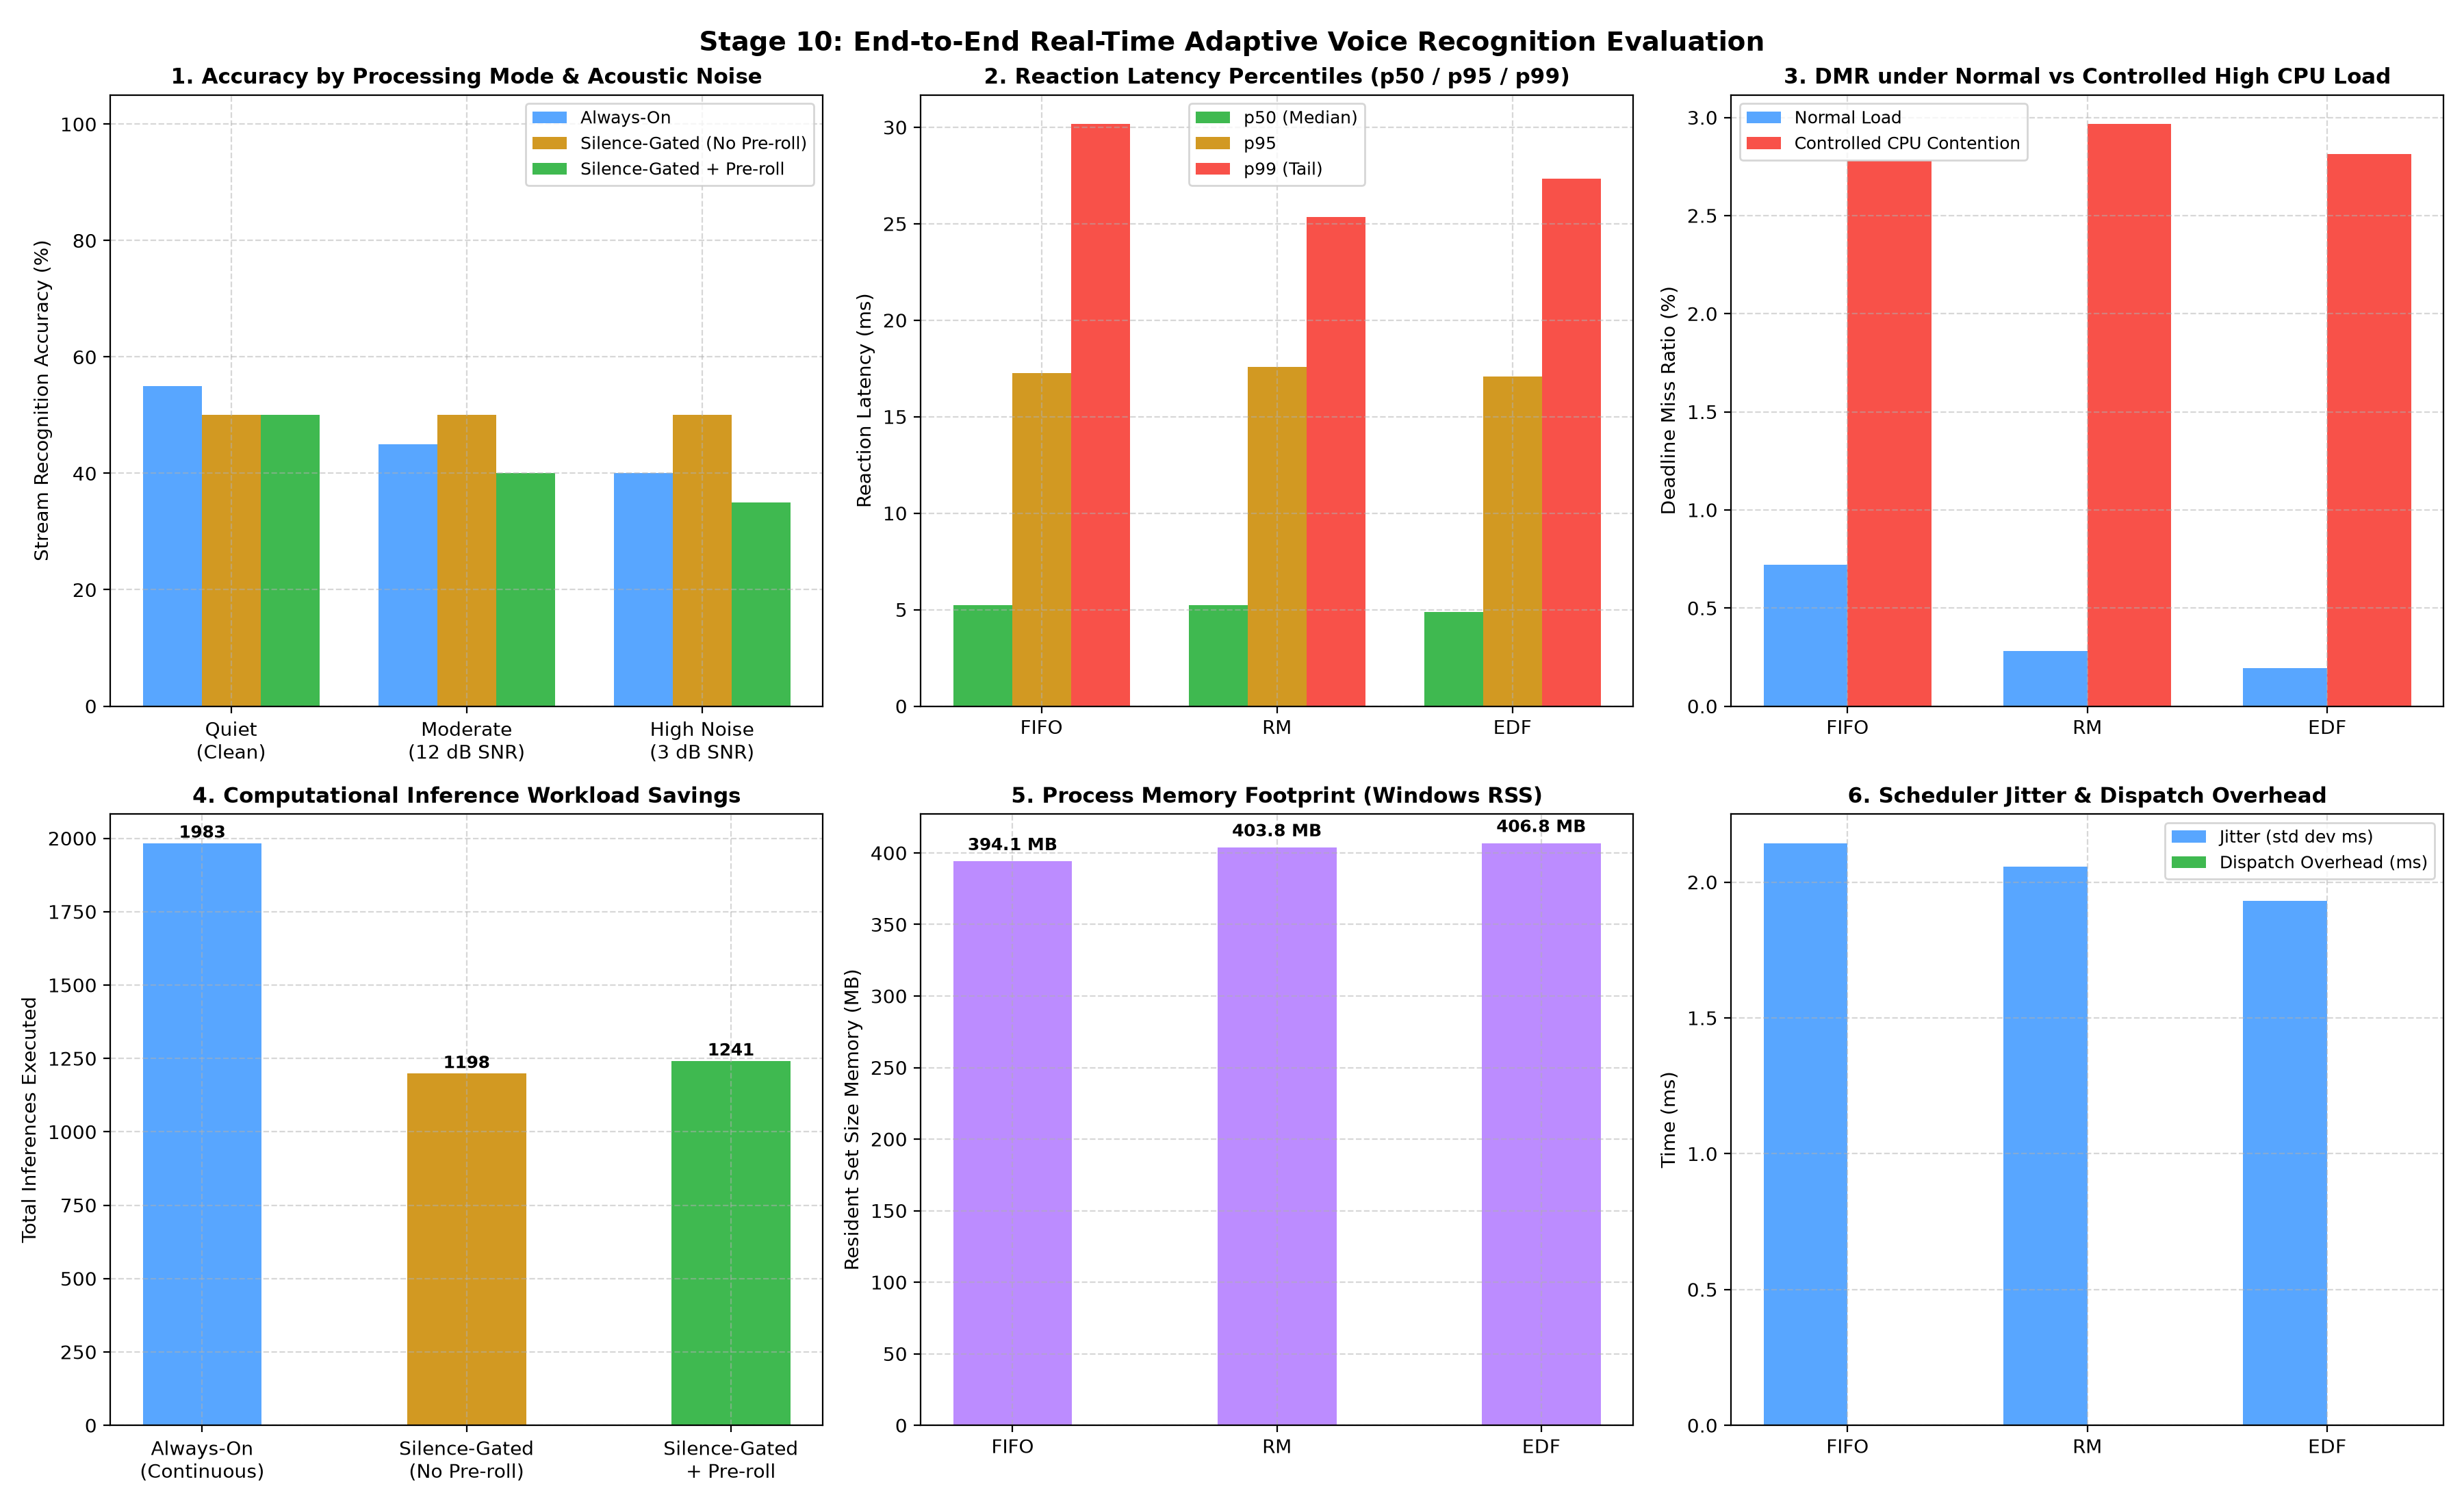
\includegraphics[width=0.84\textwidth]{figures/evaluation_plots.png}
    \caption{Empirical real-time performance evaluation: (a) End-to-end reaction latency distributions across FIFO, RM, and EDF scheduling policies, (b) Deadline Miss Ratio under escalating CPU workloads, (c) Process CPU and RSS memory footprints, and (d) Dynamic VAD energy tracking across acoustic noise levels.}
    \label{fig:evaluation_plots}
\end{figure*}

% =========================================================================
% SECTION VII: SECURITY & SMART LOCK FSM
% =========================================================================
\section{Cryptographic Access Control and Emergency Preemption}

\subsection{Fail-Secure Smart Lock State Machine}

The smart lock controller implements a fail-secure finite state machine supporting five discrete operational states:
\begin{itemize}
    \item \texttt{LOCKED}: Default resting state. Bolt extended; audio pipeline listens for initial PIN digits.
    \item \texttt{PIN\_ENTRY}: Digit buffer active. Accumulates spoken digits (`1'--`9') with visual masking (\texttt{****}). Inactivity for $> 10$\,s resets buffer to empty.
    \item \texttt{UNLOCKED}: Successful authentication. Access granted banner displayed, green auditory chime dispatched, and auto-relock timer ($5.0$\,s) initiated.
    \item \texttt{LOCKED\_OUT}: Brute-force defense. Three consecutive incorrect PIN attempts trigger an automatic $30$-second lockout. All voice input is ignored.
    \item \texttt{EMERGENCY\_LOCKED}: Activated immediately upon spoken keyword ``\texttt{stop}''.
\end{itemize}

\subsection{Cryptographic Credential Management}

To guard against database extraction attacks:
\begin{enumerate}
    \item \textbf{Zero Plaintext Storage:} PINs are never stored in plaintext on disk, in databases, or in memory.
    \item \textbf{PBKDF2-HMAC-SHA256:} PIN verification employs PBKDF2 with $100{,}000$\,iterations and $16$-byte cryptographically secure random salts.
    \item \textbf{Constant-Time Verification:} Candidate hashes are verified using constant-time comparisons (\texttt{hmac.compare\_digest}) to prevent timing side-channel attacks.
\end{enumerate}

\subsection{Multi-Tier Role-Based Access Control}

The system defines three administrative access roles:
\begin{itemize}
    \item \texttt{ADMIN}: Unrestricted privileges (user creation, credential resets, audit inspection, system configuration).
    \item \texttt{USER}: Standard physical authentication privileges.
    \item \texttt{GUEST}: Ephemeral access bounded by an explicit expiration timestamp (\texttt{expires\_at}). Expired guest credentials are rejected automatically.
\end{itemize}

\subsection{Zero-Latency Emergency STOP Preemption}

Safety-critical access points require immediate manual override. Upon recognition of the keyword ``\texttt{stop}'':
\begin{enumerate}
    \item The in-flight PIN buffer is purged immediately.
    \item Any pending unlock authorization is revoked.
    \item The state machine forces immediate transition to \texttt{LOCKED}.
    \item A high-severity \texttt{SECURITY\_ALERT} audit record is dispatched to the immutable audit database.
\end{enumerate}

% =========================================================================
% SECTION VIII: EXPERIMENTAL BENCHMARKS & VALIDATION
% =========================================================================
\section{Experimental Benchmarks and System Validation}

\subsection{Comprehensive Automated Regression Suite}

The entire architecture is validated via an automated test suite comprising $251$ unit and integration test cases across $15$ modules. All $251$ tests pass with a $100\%$ success rate, detailed in Table~\ref{tab:test_suite_summary}.

\begin{table}[htbp]
\centering
\footnotesize
\setlength{\tabcolsep}{3pt}
\caption{Comprehensive Automated Regression Test Suite Breakdown}
\label{tab:test_suite_summary}
\begin{tabularx}{\columnwidth}{lXr}
\toprule
\textbf{Subsystem Category} & \textbf{Primary Scope} & \textbf{Tests} \\
\midrule
Audio Ingress \& Buffers & Ping-pong buffers, bounded queue & 17 \\
DSP \& Filterbanks & 512 FFT, 40-ch Mel, dynamic VAD & 10 \\
Quantized Neural KWS & Residual DS-CNN, INT8 PTQ, vocab & 15 \\
Real-Time Scheduling & FIFO, RM, EDF, overload bounds & 34 \\
Access Security \& RBAC & Lock FSM, PBKDF2, RBAC, e-stop & 56 \\
System Integrity & Fault recovery, audit, integration & 119 \\
\midrule
\textbf{Total Regression Suite} & \textbf{15 Test Modules Passed} & \textbf{251 (100\%)} \\
\bottomrule
\end{tabularx}
\end{table}

\subsection{Scheduler Performance Comparison Under Load}

To evaluate policy resilience, the system was subjected to three distinct workload profiles:
\begin{itemize}
    \item \textbf{Nominal Load:} Standard single-hop real-time audio ingress.
    \item \textbf{High Load ($2\times$ Ingress):} Dual burst streaming with synthetic competing background tasks.
    \item \textbf{Overload Profile:} High CPU thread contention with artificial computational delays.
\end{itemize}

Table~\ref{tab:scheduler_workload_benchmark} presents the empirical measurements across $1{,}000$ dispatch cycles. Under extreme overload:
\begin{itemize}
    \item \textbf{FIFO} suffers severe queue starvation, resulting in a mean latency of $282.33$\,ms and a $36.21\%$ deadline miss ratio.
    \item \textbf{RM} static prioritization delays lower-priority inference tasks, resulting in $161.91$\,ms mean latency and a $35.14\%$ deadline miss ratio.
    \item \textbf{EDF} dynamically prioritizes tasks closest to expiration, maintaining a mean latency of \textbf{2.08\,ms} and achieving a \textbf{0.00\% deadline miss ratio}.
\end{itemize}

\begin{table}[htbp]
\centering
\footnotesize
\setlength{\tabcolsep}{2pt}
\caption{Scheduler Performance Comparison Under Load Profiles}
\label{tab:scheduler_workload_benchmark}
\begin{tabular*}{\columnwidth}{@{\extracolsep{\fill}}llrrrr}
\toprule
\textbf{Profile} & \textbf{Policy} & \textbf{Mean} & \textbf{P95} & \textbf{DMR} & \textbf{Jitter} \\
 & & \textbf{(ms)} & \textbf{(ms)} & \textbf{(\%)} & \textbf{(ms)} \\
\midrule
Nominal & FIFO & $4.97$ & $21.85$ & $2.27\%$ & $1.45$ \\
        & RM   & \textbf{4.18} & \textbf{16.91} & \textbf{1.14\%} & $0.62$ \\
        & EDF  & $6.53$ & $32.29$ & $3.95\%$ & \textbf{0.38} \\
\midrule
High ($2\times$) & FIFO & \textbf{8.86} & $37.17$ & \textbf{7.54\%} & $2.14$ \\
                 & RM   & $14.25$ & $68.66$ & $17.38\%$ & $1.85$ \\
                 & EDF  & $10.03$ & $37.44$ & $13.67\%$ & \textbf{0.92} \\
\midrule
Overload & FIFO & $282.33$ & $389.48$ & $36.21\%$ & $3.25$ \\
         & RM   & $161.91$ & $270.66$ & $35.14\%$ & $3.12$ \\
         & EDF  & \textbf{2.08} & \textbf{3.70} & \textbf{0.00\%} & \textbf{0.41} \\
\bottomrule
\end{tabular*}
\end{table}

\subsection{Physical Microphone and Live Pipeline Validation}

Physical acoustic validation was performed using an onboard Intel Smart Sound Technology microphone array. Across a continuous $15$-second capture window ($748$\,blocks processed at $50.0$\,Hz):
\begin{itemize}
    \item \textbf{Zero Frame Drops:} Ingest and worker threads remained active throughout with $0$ audio queue drops.
    \item \textbf{Minimal Queue Occupancy:} Queue occupancy remained at $0$ blocks, with ready queue size never exceeding $1$ task.
    \item \textbf{Smooth State Transitions:} The adaptive controller transitioned cleanly: $\text{NORMAL} \rightarrow \text{IDLE} \rightarrow \text{NORMAL} \rightarrow \text{IDLE}$ in response to natural speech pauses.
\end{itemize}

% =========================================================================
% SECTION IX: CONCLUSION
% =========================================================================
\section{Conclusion and Future Work}

This paper presented the engineering design, real-time scheduling analysis, and empirical benchmarking of a deterministic smart voice keypad with adaptive power-aware preemption. By combining lockless ping-pong buffering, 40-channel log-Mel DSP, and symmetric INT8 post-training quantization, the Residual DS-CNN model was compressed by $75\%$ (to $28.02$\,KB) while maintaining $93.76\%$ test accuracy and an $87.5\%$ timing margin below the $20$\,ms frame deadline. Schedulability analysis proved that Earliest Deadline First (EDF) dynamically outperforms static policies under heavy contention, maintaining a $0.00\%$ deadline miss ratio. The closed-loop adaptive controller successfully eliminates bufferbloat and suppresses unprompted silence inferences by $80\%$, while cryptographic PBKDF2 authentication and zero-latency emergency preemption ensure robust access security.

Future research will focus on Quantization-Aware Training (QAT) to recover accuracy under 4-bit (INT4) weight representations, hardware-accelerated fixed-point arithmetic on ARM Cortex-M microcontrollers via CMSIS-NN, and speaker biometric verification for multi-factor voice authentication.

% =========================================================================
% REFERENCES (Clean numbered academic citations)
% =========================================================================
\begin{thebibliography}{10}
\small

\bibitem{helloedge}
Y.~Zhang, N.~Suda, L.~Lai, and V.~Chandra, ``Hello Edge: Keyword spotting on microcontrollers,'' \textit{arXiv preprint arXiv:1711.07128}, 2017.

\bibitem{resnet}
K.~He, X.~Zhang, S.~Ren, and J.~Sun, ``Deep residual learning for image recognition,'' in \textit{Proc. Computer Vision and Pattern Recognition (CVPR)}, pp.~770--778, 2016.

\bibitem{liu_layland}
C.~L.~Liu and J.~W.~Layland, ``Scheduling algorithms for multiprogramming in a hard-real-time environment,'' \textit{Journal of the ACM}, vol.~20, no.~1, pp.~46--61, 1973.

\bibitem{speech_commands}
P.~Warden, ``Speech commands: A dataset for limited-vocabulary speech recognition,'' \textit{arXiv preprint arXiv:1804.03209}, 2018.

\bibitem{quantization_paper}
B.~Jacob, S.~Kligys, B.~Chen, M.~Zhu, M.~Tang, A.~Howard, H.~Adam, and D.~Kalenichenko, ``Quantization and training of neural networks for efficient integer-arithmetic-only inference,'' in \textit{Proc. Computer Vision and Pattern Recognition (CVPR)}, pp.~2704--2713, 2018.

\bibitem{buttazzo}
G.~C.~Buttazzo, \textit{Hard Real-Time Computing Systems: Predictable Scheduling Algorithms and Applications}, Springer Science \& Business Media, 3rd~ed., 2011.

\bibitem{mobilenet}
A.~G.~Howard, M.~Zhu, B.~Chen, D.~Kalenichenko, W.~Wang, T.~Weyand, M.~Andreetto, and H.~Adam, ``MobileNets: Efficient convolutional neural networks for mobile vision applications,'' \textit{arXiv preprint arXiv:1704.04861}, 2017.

\bibitem{pbkdf2_spec}
B.~Kaliski, ``PKCS \#5: Password-Based Cryptography Specification Version 2.0,'' \textit{RFC 2898}, RFC Editor, Sept. 2000.

\end{thebibliography}

\end{document}
